
\begin{figure}[]
    \centering
    \begin{subfigure}[t]{0.48\linewidth}
        \centering        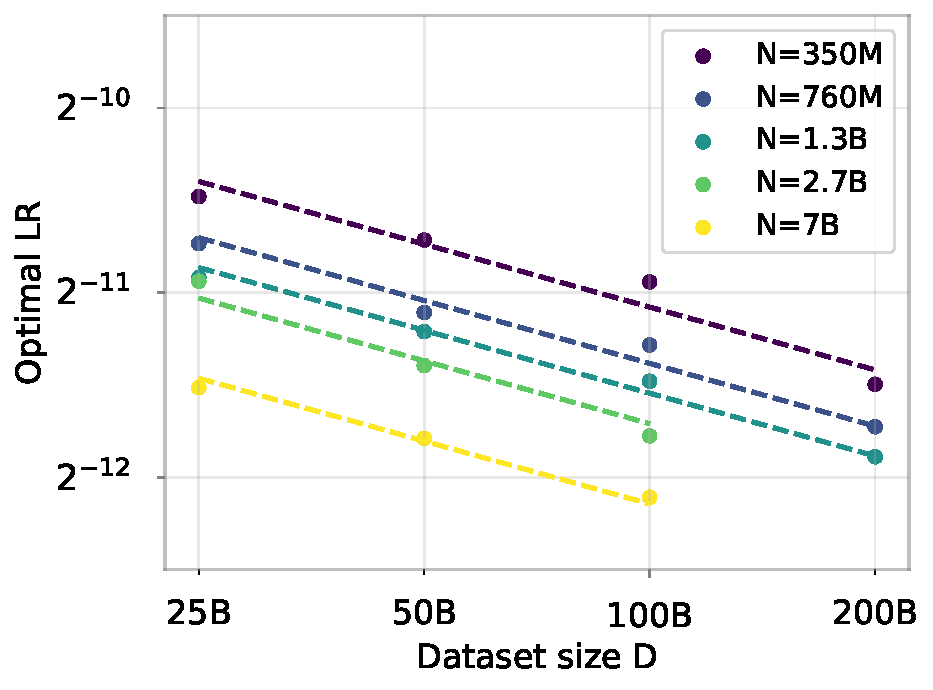
\includegraphics[width=\linewidth]{images/opt_lr_d_n.pdf}
        \caption{}
        \label{fig:opt_lr_d_n}
    \end{subfigure}
    \begin{subfigure}[t]{0.48\linewidth}
        \centering
        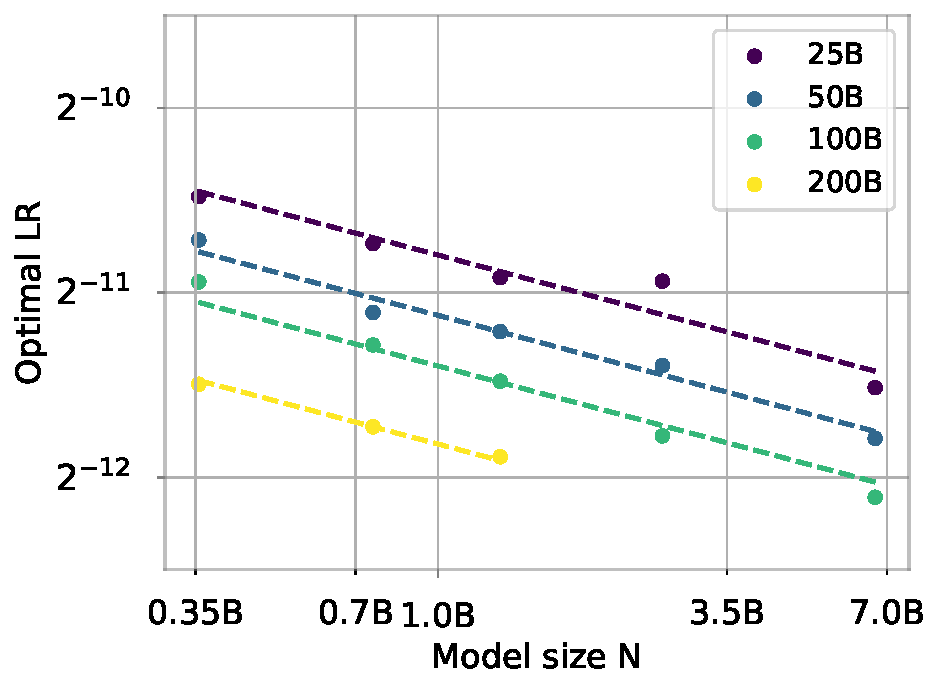
\includegraphics[width=\linewidth]{images/opt_lr_n_d.pdf}
        \caption{}
        \label{fig:opt_lr_n_d}
    \end{subfigure}
    \caption{\textbf{(a)} There is a linear relationship between $\log D$ and $\log \optlr$ for different model sizes $N$. \textbf{(b)} There is a linear relationship between $\log N$ and $\log \optlr$ for different values of dataset size $D$.}
\vspace{-0.3cm}
\end{figure}


\section{Scaling Law with respect to model size}


So far we have considered \Cref{eq:powerlaw} with constants fitted independently for each model size. Fully determining the joint scaling properties of the model architecture and token horizon is outside of the scope of this paper -- doing so would be computationally infeasible. Nonetheless, we will here provide some preliminary results and discussions regarding a scaling law for both model size $N$ and token horizon $D$. In \Cref{fig:opt_lr_n_d} we plot the optimal LR as a function of $N$, and in \Cref{fig:opt_lr_d_n} we plot it as a function of $D$. Both curves are straight lines when the axes are logarithmic. This observation motivates the following functional form, which is mathematically derived in \Cref{appendix:derivation}.
\begin{equation}
\label{eq:scaling_law}
   \optlr(N,D)=C N^{-\alpha} D^{-\beta}
\end{equation}
Here, the constant $C$ is the ideal learning rate for a model of size $1B$ and token horizon $1B$, where the precise numerical value of $C$ may depend on the batch size (see section \ref{sec:bs}), vocabulary size and tokenization. The factor $N^{-\alpha}$ captures the fact that the optimal LR decreases with model size $N$, while the factor $D^{-\beta}$ captures that optimal LR also decreases with token horizon $D$. We now fit \Cref{eq:scaling_law} to our data for the models of size 760m, 1.3B, and 2.7B, using the 7B model of \Cref{sec:llama_case_study} as a held-out validation set. We use the huber loss with $\delta=\e{1}{-3}$ and the BFGS algorithm, similar to \cite{hoffmann2022training}. We observe a good fit with RMSE$=\e{2.2}{-5}$ and a validation $R^2$ of $0.978$. The numerical values we find are:
\begin{equation}
\label{eq:final_numbers}
C\sim\e{1.55}{-3}, \quad \alpha\sim0.23, \quad \beta\sim0.32
\end{equation}
We depict the results in \Cref{fig:opt_lr_scaling_law}. For smaller models (mainly 50m and 125m) a larger $\beta$ is observed from the experiments. We thus consider \Cref{eq:scaling_law} to be valid in the regime of large models ($\geq$ 760M parameters).









\begin{figure}[]
\begin{center}
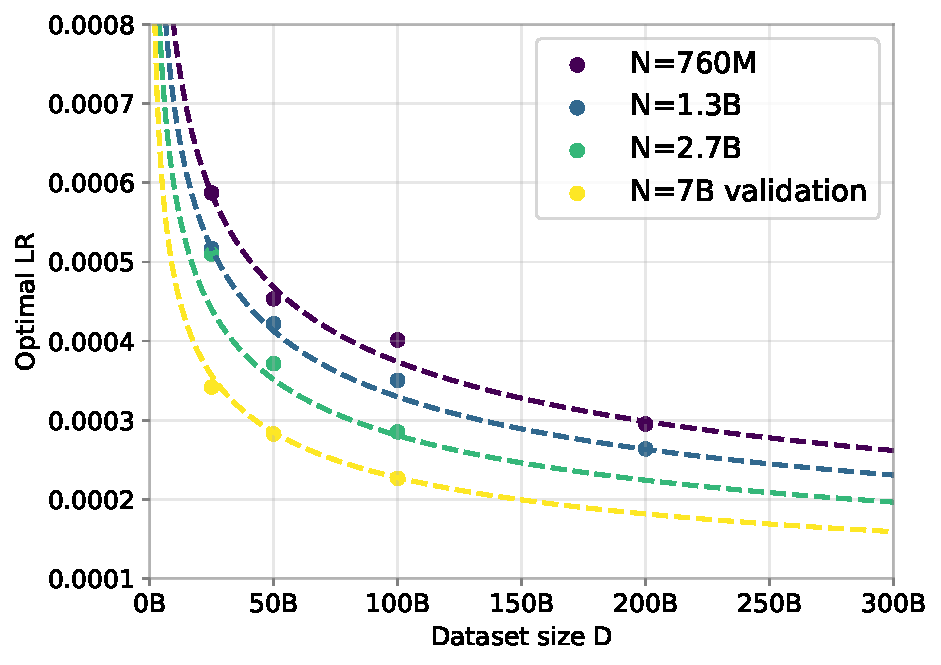
\includegraphics[width=0.6\textwidth]{images/opt_lr_scaling_law.pdf}
\vspace{-0.3cm}
\caption{Fit of  \Cref{eq:scaling_law} compared to the experimental results. The data points for the 7B model of \Cref{sec:llama_case_study} are excluded at the time of fitting and used as validation data. We have an $R^2$ of $0.978$ on this validation data. \rebuttal{Note, the 7B model uses the Llama architecture while the other data points use the GPT-3 architecture. This experiment thus demonstrates that the scaling laws have predictive power across model architectures.}}
\label{fig:opt_lr_scaling_law}
\vspace{-0.3cm}
\centering
\end{center}
\end{figure}

